\documentclass[landscape,a0paper,fontscale=0.305]{baposter}

\usepackage{times}
\usepackage{graphicx}
\usepackage{amsmath,amssymb}
\usepackage{booktabs}
\usepackage{colortbl}
\usepackage{xcolor}
\usepackage{multicol}
\usepackage{tikz}
\usetikzlibrary{arrows.meta,positioning,shapes.geometric}

\definecolor{ctitle}{HTML}{2c2739}
\definecolor{mypurple}{HTML}{d2cce1}
\definecolor{myteal}{HTML}{1f9ea8}
\definecolor{mybg}{HTML}{f7f7fb}

\begin{document}

\begin{poster}{
    grid=false,
    columns=6,
    colspacing=1.0em,
    headerColorOne=mypurple!95,
    borderColor=mypurple,
    textborder=faded,
    headerborder=open,
    headershape=roundedright,
    headershade=plain,
    background=none,
    bgColorOne=mybg,
    headerheight=0.18\textheight
}
{}
{\sc\Huge\bf\textcolor{ctitle}{LVForge: PE Malware Detection}\\[0.15em]
\sc\LARGE\bf\textcolor{ctitle}{Transformer + Deep Metric Learning}}
{\Large Ly Ngoc Vu\\[0.2em]
\normalsize Industrial University of Ho Chi Minh City}
{}

\headerbox{\bf\color{ctitle} Problem \& Motivation}{name=problem,column=0,row=0,span=2}{
\begin{itemize}
\item Windows PE malware detection needs \textbf{high recall} at \textbf{low false-positive rate}.
\item Standard accuracy alone is insufficient for deployment.
\item Class imbalance (benign:malware \(\approx 1:19\)) makes threshold behavior critical.
\end{itemize}

\textbf{Goal:} build an operationally robust detector using a shared Transformer and compare objective functions.
}

\headerbox{\bf\color{ctitle} Contributions}{name=contrib,column=2,row=0,span=2}{
\begin{itemize}
\item Unified Flax/JAX pipeline for baseline + DML variants.
\item Controlled comparison of \texttt{baseline}, \texttt{arcface}, \texttt{contrastive}, \texttt{triplet}, \texttt{multi\_similarity}.
\item Multi-seed evaluation with operational metric: \(\mathrm{TPR@FPR}=10^{-2}\).
\item Architecture-level extension of LVModel with metric-learning heads.
\end{itemize}
}

\headerbox{\bf\color{ctitle} Data \& Setup}{name=setup,column=4,row=0,span=2}{
\begin{itemize}
\item Dataset size: \textbf{34,370} PE samples.
\item Input: text-like PE features, labels \{benign, malware\}.
\item Backbone config: \(d_{model}=256\), heads\(=8\), FFN\(=512\), layers\(=2\), max seq len\(=380\).
\item Training: batch\(=128\), epochs\(=5\), LR\(=2\times 10^{-4}\), dropout\(=0.1\).
\end{itemize}
}

\headerbox{\bf\color{ctitle} Unified Pipeline}{name=pipeline,column=0,below=problem,span=3}{
\begin{center}
\resizebox{0.94\textwidth}{!}{%
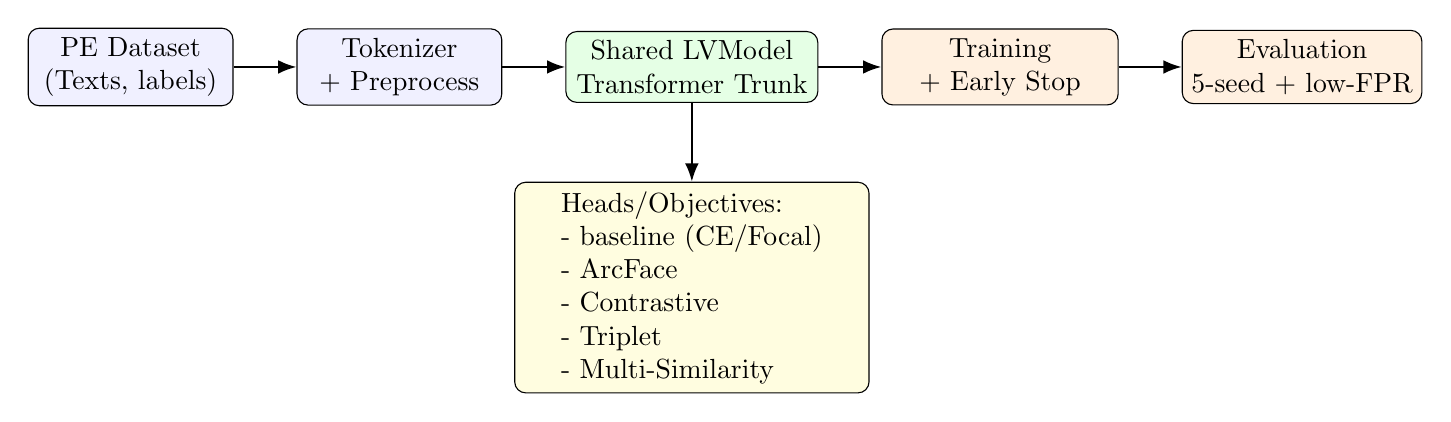
\begin{tikzpicture}[
  node distance=7mm and 8mm,
  stage/.style={draw, rounded corners, minimum width=26mm, minimum height=9mm, align=center, fill=blue!6},
  core/.style={draw, rounded corners, minimum width=32mm, minimum height=9mm, align=center, fill=green!10},
  block/.style={draw, rounded corners, minimum width=45mm, minimum height=15mm, align=left, fill=yellow!12},
  evalbox/.style={draw, rounded corners, minimum width=30mm, minimum height=9mm, align=center, fill=orange!12},
  arr/.style={-Latex, thick}
]
\node[stage] (d) {PE Dataset\\(Texts, labels)};
\node[stage, right=of d] (p) {Tokenizer\\+ Preprocess};
\node[core, right=of p] (b) {Shared LVModel\\Transformer Trunk};
\node[block, below=10mm of b] (h) {Heads/Objectives:\\- baseline (CE/Focal)\\- ArcFace\\- Contrastive\\- Triplet\\- Multi-Similarity};
\node[evalbox, right=of b] (t) {Training\\+ Early Stop};
\node[evalbox, right=of t] (e) {Evaluation\\5-seed + low-FPR};

\draw[arr] (d)--(p);
\draw[arr] (p)--(b);
\draw[arr] (b)--(t);
\draw[arr] (t)--(e);
\draw[arr] (b)--(h.north);
\end{tikzpicture}
}
\end{center}
}

\headerbox{\bf\color{ctitle} LVModel Architecture Details}{name=arch,column=3,below=setup,span=3}{
\textbf{Base LVModel:}
\begin{itemize}
\item Input shape: \((B,T,d)\); token + positional embedding:
\(\mathbf{H}_0 = E_{tok}(\mathbf{X}) + E_{pos}(1{:}T)\).
\item MHA uses one combined QKV projection:
\(\mathrm{QKV}=W_{qkv}\mathbf{H}\), reshaped to \(Q,K,V\) by heads.
\item Scaled dot-product attention:
\(\mathrm{softmax}(QK^\top/\sqrt{d_h})\), then output projection.
\item \textbf{Pre-norm} encoder layer:
\(x \leftarrow x + \mathrm{MHA}(\mathrm{LN}(x))\),
\(x \leftarrow x + \mathrm{FFN}(\mathrm{LN}(x))\).
\item LVModel head:
mean-pool \(\rightarrow\) dense+tanh \(\rightarrow\) dropout \(\rightarrow\) LN \(\rightarrow\) classifier logits.
\end{itemize}

\textbf{Metric extensions:}
\begin{itemize}
\item Shared trunk \(\rightarrow\) projection to \(d_{emb}=256\) \(\rightarrow\) LayerNorm + \(\ell_2\)-norm embedding.
\item ArcFace head: angular margin \((m=0.5, s=64)\).
\item Contrastive/Triplet/MS: linear logits + auxiliary metric losses.
\end{itemize}
}

\headerbox{\bf\color{ctitle} Main Results (5-seed mean)}{name=results,column=0,below=pipeline,span=4}{
\begin{center}
\renewcommand{\arraystretch}{1.3}
\setlength{\tabcolsep}{10pt}
\begin{tabular}{lccccc}
\toprule
\rowcolor{mypurple!45}
\textbf{Variant} & \textbf{Accuracy} & \textbf{F1} & \textbf{ROC-AUC} & \textbf{PR-AUC} & \textbf{TPR@FPR=1e-2} \\
\midrule
baseline & 0.9924 & 0.9960 & 0.9983 & 0.9999 & 0.9754 \\
arcface & 0.7979 & 0.7934 & 0.9704 & 0.9984 & 0.0000 \\
contrastive & 0.9931 & 0.9964 & 0.9971 & 0.9997 & 0.9533 \\
triplet & 0.9932 & 0.9964 & 0.9969 & 0.9998 & 0.9351 \\
\rowcolor{cyan!12}
multi\_similarity & \textbf{0.9946} & \textbf{0.9972} & 0.9978 & 0.9999 & \textbf{0.9851} \\
\bottomrule
\end{tabular}
\end{center}

\vspace{0.4em}
\textbf{Runtime (single run):} baseline 107.1s, arcface 93.6s, contrastive 130.8s, triplet 132.6s, multi\_similarity 128.3s.
}

\headerbox{\bf\color{ctitle} Discussion \& Takeaways}{name=take,column=4,below=arch,span=2}{
\begin{itemize}
\item DML improves performance, but \textbf{objective selection matters}.
\item \textbf{Multi-Similarity} is the best overall operating point.
\item Baseline remains a strong competitor.
\item ArcFace is unstable at strict low-FPR thresholds in this setup.
\end{itemize}

\textbf{Deployment recommendation:}
Use Multi-Similarity as primary model, baseline as fallback/reference, and calibrate thresholds for target FPR.
}

\headerbox{\bf\color{ctitle} Reproducibility}{name=repro,column=0,below=results,span=6}{
Code and paper assets are in: \texttt{/root/LVForge/docs/paper/}\\
Main paper: \texttt{IEEE-conference-template-062824/IEEE-conference-template-062824.tex}\\
All variants executed via: \texttt{scripts/run\_all.py} with recorded logs and aggregated JSON metrics.
}

\end{poster}
\end{document}
